\chapter{Implementation and Testing}
This chapter will explain the implementation choices of the various applications built in this thesis. 
It will also be presented how these applications will be tested.

\section{Installing NDN}

\gls{ndn-cxx}

\gls{NFD}

\gls{PyNDN2}

\gls{IBC}~\cite{charm13}

\gls{PBC}~\cite{ben2007implementation}


\section{FileSync.py application}
Application goal explained in~\autoref{file-sync}
Appendix code~\autoref{apx:file-sync-code}

FileSync is a python application that will synchronize all files in a specified path, with all participants within the synchronization room.

\section{Application.py}
Application flow explained in~\autoref{sensor-application}

Device code~\autoref{apx:device-code}
\gls{PKG} code~\autoref{apx:pkg-code}

Main code~\autoref{apx:main-code}

\subsection{Packet Design}
Initialization packets have the structure presented in~\autoref{fig:init_interest-data}.
Initially the idea was to have the \textit{\gls{TMPK}} appended to the Content Name. 
However I experienced a problem where the Init Data never arrived at destination node. 
After some research in \texttt{ndn-cxx} documentation I found that the packets have a \texttt{MAX\_NDN\_PACKET\_SIZE} of 8800 bytes and the Init Data exceeded this limit and reached 8904 bytes.
Because the \gls{TMPK} is approximately 2\gls{KB} and was appended to the Content Name in the Interest, the Data response off course had to have the same Content Name, hence 2\gls{KB} overhead in the Name. 
The \gls{TMPK} can as easily be appended to the KeyLocator Name, hence the Data response can be 2\gls{KB} less, resulting to a 6866 bytes Init Data packet.

Sensor packets have the structure presented in~\autoref{fig:sensor_interest-data}.
\begin{description}
	\item[Init Interest] - 
  The initialization Interest seen in~\autoref{fig:init_interest-data}
  KeyLocator can be of type Name. 
  As described in the \gls{NDN} Packet Format~\cite{ndnpacketformat}, generally this field can be used to specify where to download the certificate used to sign the Interest.
  However, in our trust model we use this field to publish the requesters Name, i.e. the requesters public key. 
  This is very useful when using \gls{IBE} and \gls{IBS}.
	\item[Init Data] - 
  The Data response the the initialization Interest contains data with a structure defined in~\autoref{apx:msgBuf-code} and illustrated in~\autoref{fig:init_interest-data}.
	\item[Sensor Interest] -
	As in the initialization Interest the KeyLocator field is used to define the requesters Name. ~\autoref{fig:sensor_interest-data}
	\item[Sensor Data] - 
  The Data response to the Sensor Interest uses the same structure as the initialization Data. It is illustrated in~\autoref{fig:sensor_interest-data}
\end{description}

\begin{figure}[ht]
  \centering
  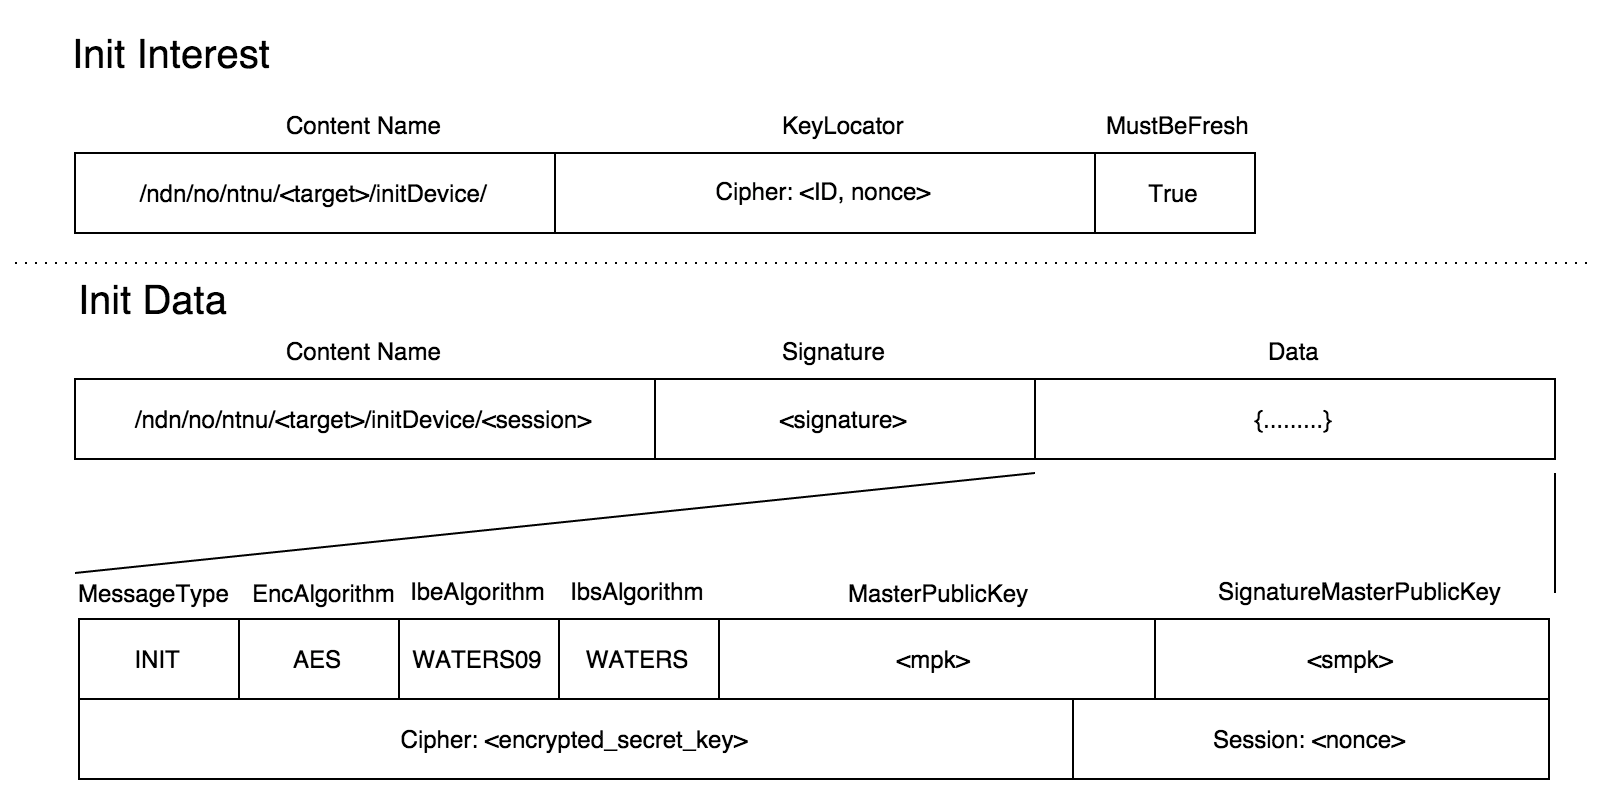
\includegraphics[width=1\textwidth]{init_interest-data.png}
  \caption{Initialization Interest and Data}
  \label{fig:init_interest-data}
\end{figure}

\begin{figure}[ht]
  \centering
  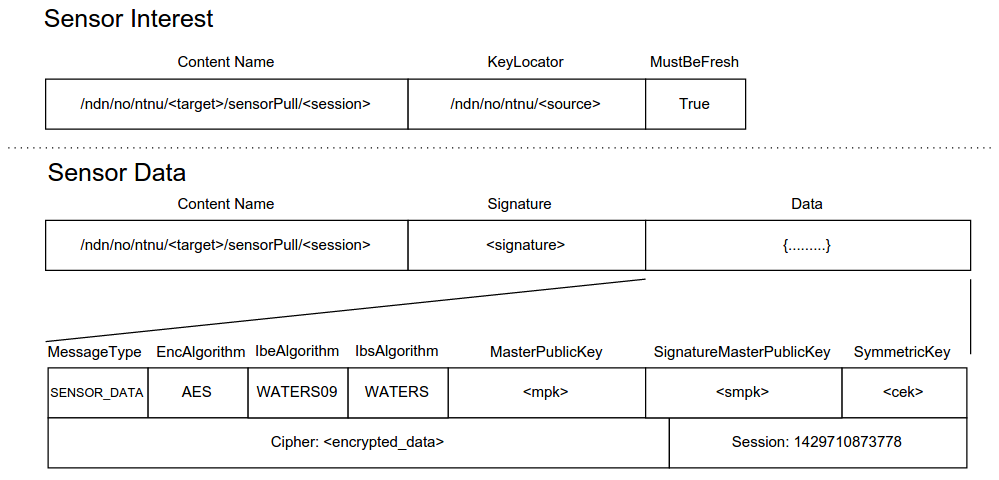
\includegraphics[width=1\textwidth]{sensor_interest-data.png}
  \caption{Sensor Interest and Data}
  \label{fig:sensor_interest-data}
\end{figure}

\section{Identity-Based Cryptography in Python}
\gls{IBE} code~\autoref{apx:ibe-code} implements two \gls{IBE} schemes and 

\begin{description}
  \item[Waters05]~\cite{DBLP:journals/iacr/Naccache05} that is a variant of Brent Waters \gls{IBE} scheme~\cite{DBLP:journals/iacr/Waters04}, but with smaller key size, hence more practical.
  \item[Waters09]~\cite{DBLP:conf/crypto/Waters09} that is also a fully secure implementation of \gls{IBE} scheme.
\end{description}

It also implements the \gls{IBS} scheme Waters presented in~\cite{DBLP:journals/iacr/Waters04}. 

\subsection{Charm - A Framework for Rapidly Prototyping Cryptosystems}
~\cite{charm13}
\subsubsection{Modifications in Charm Library}
CHARM: pksigwaters.py

\subsection{Modifications in PyNDN2}
PyNDN2: added IB signature


